\section{Bisection Games}

The tree produced in this fashion will be the same for all honest parties, since they agree on
the epochs, slot leader public keys, and signatures. The only difference between two honest parties
can be that one honest party may have transitioned to epoch $j+1$, while another is still in epoch
$j$. However, this difference cannot span more than one epoch.

Consider now a handover tree produced by the adversary, and let us compare it to a handover tree
computed by an honest party. 

The verifier requests from
the provers a Merkle Tree~\cite{merkle} commitment to the history of stake evolution of
the protocol. The provers send their respective commitments to the verifier. The verifier
then forwards the commitment of each prover to the other provers, allowing them to
challenge the statement of their peers. This challenge takes the form of a bisection
game, in which one path of the Merkle Tree is traversed until a leaf is reached.
When a leaf is reached, an adversarial prover will be discovered, as she will fail to provide
the required evidence of epoch transition. 

The verifier is interacting with a set of provers $\mathcal{P}$, which he has to sort through.
After receiving all the proofs $(\pi_i, n_i)$ by the provers,
this task is simplified by interacting with them sequentially in pairs,
in a tournament fashion. The verifier
begins by choosing two arbitrary provers $P_1$ and $P_2$ from the set $\mathcal{P}$
(in case $|mathcal{P} = 1$ the decision of the verifier is trivial). The
verifier \emph{pits one against the other} by facilitating a game between
$P_1$ and $P_2$ and decides which of the
two provers wins. He then rejects the loser and chooses a new prover from the
set $\mathcal{P}$ to compete against the winner. This process continues until
there is only one champeion prover left. The champion's Merkle tree $\pi$ is adopted
as the correct one.

\begin{figure*}[h]
    \centering
    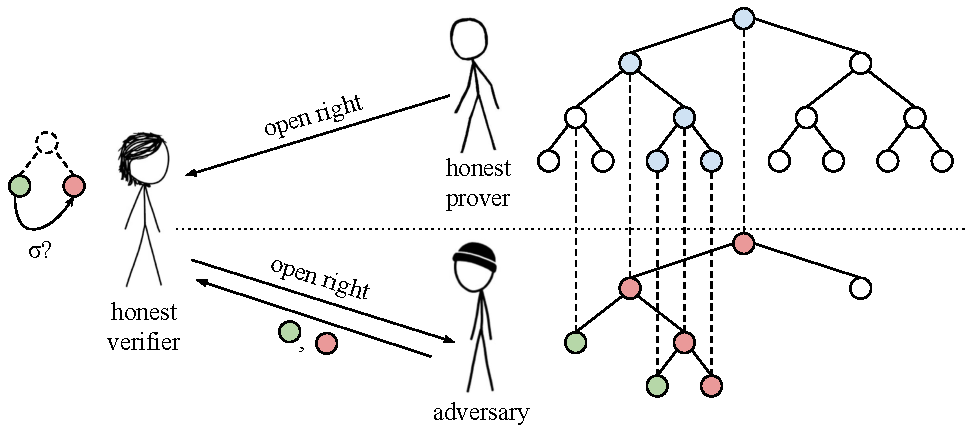
\includegraphics[width=0.55 \textwidth,keepaspectratio]{figures/bisection-game.pdf}
    \caption{The honest prover, here the attacker, and the adversarial prover,
             here the defender, in the PoPoS bisection game. Challenges to \emph{open
             left} or \emph{open right} are relayed by the honest verifier.}
    \label{fig.bisection-game}
\end{figure*}

\import{./}{algorithms/alg.verifier}
\import{./}{algorithms/alg.prover}
